\chapter{Related Work
    \pgsize{15 p.}
}
\label{chap:relatedwork}

\mnote{Related work on goal and methodology}
Collaboration is a key factor in software engineering processes and especially \gls{MDSD}, but it also represents a key challenge, in particular due to the necessity of consistency preservation~\cite{franzago2018mdseChallenges-TSE}.
This thesis contributes to the goal of preserving consistency of different engineering artifacts or models, and it especially uses and extends the methodology of model transformations to achieve that goal.
We relate our research to existing work separated into two categories given by the general goal of consistency preservation, which primarily comprises different approaches to solve the underlying problem but with potentially different methodologies, and the methodology of using transformations for consistency preservation and specific topics regarding transformations, their properties, and their composition.

\begin{figure}
    \centering
    \begin{tikzpicture}[every node/.append style={font=\footnotesize}]

\draw[fill=darkred!10] (0.8em,0.5em) ellipse (3em and 3em);

\draw[darkgreen, thick] (0,0) ellipse (15em and 15em);
\node[darkgreen, anchor=north, align=center, font=\footnotesize\bfseries] at (0, 14em) {\emph{Goal:}\\ Consistency and its Preservation};
\draw[darkgreen, thick] (3em,-0.25em) ellipse (11.5em and 11.5em);
\node[darkgreen, anchor=north, align=center, font=\footnotesize\bfseries] at (3em, 10.25em) {\emph{Methodology:}\\ Consistency by Transformation};
\draw (-6.5em,4.5em) ellipse (7.5em and 3.5em);
\node[anchor=west, align=center] at (-12.5em, 5em) {View-Update\\ Problem};
\draw (-7em,-1em) ellipse (7.5em and 3.5em);
\node[anchor=west, align=center] at (-14em, -1em) {Traceability /\\ Model Merging};
\draw (-4em,-7em) ellipse (5.5em and 7em);
\node[anchor=south, align=center] at (-4em, -13.5em) {Constraint Solving /\\ Model Finding};
\draw (-2.5em,2em) ellipse (4.5em and 5em);
\node[anchor=center, align=center] at (-3.5em, 4em) {Commonalities\\ Approaches};
\draw (5em,3.5em) ellipse (6em and 3.5em);
\node[anchor=north, align=center] at (5.5em, 6.5em) {Transformation\\ Composition and Chains};
\draw (5em,0.5em) ellipse (7em and 3.5em);
\node[anchor=north, align=center] at (5.5em, 3.75em) {Transformation\\ Networks};
\draw (4.5em,-4.5em) ellipse (7.5em and 6em);
\node[anchor=south, align=center] at (4.7em, -10.25em) {Multidirectional\\ Transformations};
\draw (4.5em,-3.5em) ellipse (7em and 4.5em);
\node[anchor=south, align=center] at (4.6em, -7.75em) {Bidirectional\\ Transformations};
\draw (4.5em,-2.5em) ellipse (6.5em and 3em);
\node[anchor=south, align=center] at (4.5em, -5.25em) {Synchronizing\\ Transformations};

\draw[darkred, thick] (0.8em,0.5em) ellipse (3em and 3em);

\end{tikzpicture}

    %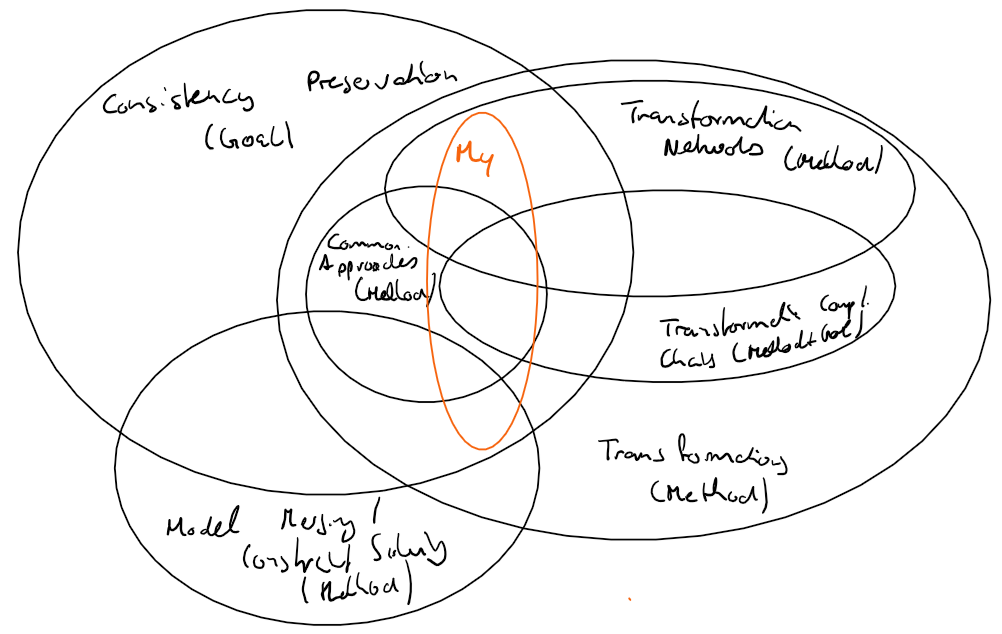
\includegraphics[width=\textwidth]{figures/epilogue/relatedwork/research_areas.png}
    \caption[Overlaps of related research areas]{Sketch of different research areas (circles) related to the work of this thesis, their overlaps, and the relation to contributions of this thesis (shaded red in the center).}
    \label{fig:relatedwork:areas}
\end{figure}

\mnote{Relations of topics}
\autoref{fig:relatedwork:areas} depicts an overview of the topics and research areas that we relate our work to and sketches how they are related to each other and to our contributions, indicated by overlaps of the ellipses representing them.
The figure is neither complete nor do the sizes of the areas and overlaps have a specific meaning.
We do also not depict the relation of each of our contributions to related topics in that figure, but we do so in the subsequent sections.
Several research topics are cross-cutting, such that some work fits into multiple categories.
We discuss these works in the areas to which they are mostly related.
Parts of the discussions in this chapter have already been published in previous work~\owncite{klare2018docsym, klare2019icmt, klare2019models, klare2020compatibility-report, klare2021Vitruv-JSS}.


%%%%
%% CONSISTENCY AND ITS PRESERVATION
%%%%
\section{Consistency and its Preservation}

\mnote{Generality of consistency}
Checking and preserving consistency of software artifacts, i.e., models, has been researched in several contexts.
It covers a broad topic and is often traced back to the \emph{view-update problem}, which considers the backpropagation of changes within a view to the original source and is especially known from database engineering~\cite{bancilhon1981viewUpdate-TDS}.
Consistency has been considered for different development artifacts, including the common scenario of \emph{roundtrip engineering} between \gls{UML} models and code~\cite{dantas2005umlsync-ISPSE}, and especially rose with the definition of a general methodology defined by the \gls{MDA} process~\cite{mda}.
Depending on the scenario, the kinds of dependencies and inconsistencies between multiple models can vary and have been discussed by \textcite{kolovos2008a}. 
Several approaches provide domain-specific solutions for consistency problems, such as for consistency between SysML~\cite{sysml} and AUTOSAR~\cite{scheid2015autosar} in the automotive domain~\cite{giese2010a}.

\mnote{Model consistency approaches}
The development of modeling frameworks, such as the \gls{EMF}~\cite{steinberg2009emf}, have enabled the definition of tools, such as transformation languages, that are independent from the actual metamodels to consider consistency between.
General methods and approaches regarding model consistency have been based on such modeling frameworks and can be separated into approaches that are only able to check consistency of models~\cite{reder2012incrementalchecking} and those that are also able to preserve or enforce it.
Consistency-preserving approaches range from providing recommendations for repair~\cite{ohrndorf2018repairRecommendataions-ICSE} over generation and classifications of repair options~\cite{kretschmer2018repairDiscovery-ICSE} to approaches that actually perform \emph{model repair}, which have been subject to intensive research and surveyed by \textcite{macedo2017ModelRepairClassification-TSE}.
The survey also classifies approaches regarding their support for the scenario of keeping multiple, i.e., more than two, models consistent, which is the focus of this thesis.
It found that only one of the considered approaches is able to handle multiple models, which is done by considering consistency pairwise, like we do in our work.

\mnote{Focus on preservation}
We focus the discussion of related work on consistency preservation rather than checking, as the contributions of this thesis aim to support it.
We first depict an overview of relevant consistency preservation approaches, including the foundation of the view-update problem, model merging, constraint solving, and the methodology of multi-view modeling.


\subsection{The View-Update Problem}

\mnote{View update in databases}
The \emph{view-update problem} is common in software engineering.
It occurs whenever a view, i.e., a model, is supposed to represent information from some underlying source, which in our case is also a model, such that modifications to this view can be propagated back to the underlying source without changing information that is not contained in the view.
The problem was and is a central topic in database research~\cite{bancilhon1981viewUpdate-TDS, dayal1982viewUpdate-TDS}, where views are derived from database tables.
Updating database tables with changes in views to them, denoted as \emph{update translation}~\cite{bancilhon1981viewUpdate-TDS}, can be achieved by considering a \emph{complement} view that contains all information of the database that is not contained in the modified view.
This means that the Cartesian product of the functions for generating a view and its complement must be injective.
Calculating the update of the database after changes to the view can be achieved by inverting this function.
There are many possible complements to a view, but for considering a view \emph{updatable}, it must be possible to translate its 
updates to the database tables with a constant complement~\cite{bancilhon1981viewUpdate-TDS}.
Update translation must, however, ensure that it leaves invariant the information in the complement.
It is thus inevitable to design views and complements properly to enable automated translation of updates.

\mnote{Lenses framework}
An application of the view-update problem to software artifacts and, in particular, to transformations, is given by the \emph{lenses} framework~\cite{foster2005Combinators-POPL, foster2007combinators-TPLS}.
It defines two essential operations, which are \emph{get} for deriving a view from a model and \emph{putback} for propagating changes in the view back to the model.
This defines a transformation between a view and an underlying model.
Specific laws ensure that lenses are \emph{well-behaved}~\cite[Def.~3.2]{foster2007combinators-TPLS}, i.e., that they are complete such that all information changed in a view is propagated back to the model, and that they do not perform unintended changes.
The proper design of the \emph{putback} function influences expressiveness and robustness of the view and the changes that can be propagated back to the underlying source~\cite{foster2007combinators-TPLS}.
Lenses also depict a well-researched formal foundation to express and study incremental transformations~\cite{stevens2008bxalgebraic-ICGT}.

\mnote{Delta lenses}
While lenses originally consider states of models, \emph{delta lenses}~\cite{diskin2011StateToDeltaSymmetric-MODELS} consider the application to deltas, which conforms to our notion of changes and consistency preservation according to \autoref{def:consistencypreservationrule}.
They particularly consider the so called \emph{symmetric} case~\cite{diskin2011StateToDeltaSymmetric-MODELS}, in which the view is not a projection from the underlying source, but the view and the underlying source are both models with information that is unique to each of them, and thus transformations are defined in both directions.

\mnote{Multiary lenses}
Lenses have also been extended to the multiary case, in which more than two models need to be kept consistent~\cite{diskin2018MultiModelSynchronization-FASE}.
It especially reflects that transformations may need to change the originally modified models as well, which is denoted as \emph{reflective updates} in that work and which we have also motivated and introduced with the notion of \emph{synchronizing transformations} in \autoref{chap:synchronization}.
Despite these multiary lenses, work on lenses is especially focused on or related to bidirectional transformations, which build the basis for our work of constructing networks of them.


\subsection{Traceability and Model Merging}

\mnote{Checking consistency}
Traceability is an important concept for different concerns, ranging from comprehension over change impact analysis to the identification and resolution of inconsistencies.
For example, architectures based on correspondence models to identify that elements belong together and affect each other among changes have been developed~\cite{szabo2013traceabilityConsistency-ASWEC}.
While traces are also used as auxiliary or witness structures for consistency preservation, much work on traceability is focused on consistency checking, such as UML/Analyzer~\cite{egyed2006umlanalyzer-ICSE} for checking consistency of \gls{UML} models incrementally, and its generalization Model/Analyzer~\cite{egyed2011modelanalyzer-TSE} for checking consistency of arbitrary models.
These tools were also extended to repair inconsistencies with repair actions derived from the incremental consistency checks to determine the scope of consistency repair~\cite{reder2012resolvingInconsistencies-ASE}.
Our approaches go beyond consistency checking and use traceability especially as a means to trace consistency relations in the practical approach realization to be able to update them among changes.

\mnote{Merging corresponding elements}
Model merging goes beyond traceability by not only providing correspondences for related information but by merging elements that share and redundantly represent information.
This process is also known as \emph{amalgamation}~\cite{koenig2017efficientConsistencyChecking-ECMFA}.
Model merging consists of matching elements that represent the same information and merging them~\cite{koenig2017efficientConsistencyChecking-ECMFA}.
Such an approach has also been applied in a framework based on category theory~\cite{diskin2010overlapsHeterogeneous-MDI}.
Model merging is comparable to the \commonalities idea (see \autoref{chap:improvement}), as it is also concerned with finding elements that represent the same information. 
Model merging is, however, usually used for merging models into a single, redundancy-free, and thus inherently consistent representation or for checking consistency during the merge task but not to preserve consistency like we do with the \commonalities approach.
In addition, \commonalities relate redundant elements by construction, i.e., as soon as an element is created that requires a corresponding one in another model, it is created, whereas model merging identifies redundant elements after their creation. 


\subsection{Multi-View Modeling}

\mnote{Consistency challenge}
Multi-view modeling, as introduced in \autoref{chap:foundations:multiview}, concerns the description of a system by means of multiple views, reflecting different interests.
A recent survey of such approaches~\cite{cicchetti2019multiview-SoSym} has identified lacking consistency management as a central challenge of them, which is also emphasized by \textcite{reineke2019ProblemMultiView-SoSym}.
In addition to identifying this challenge, \textcite{persson2013characterizationMultiView-EMSOFT} classify different types of relations between views to be distinguished.
Our contributions can be applied in the context of multi-view modeling, as model transformations are a possible means to solve the consistency challenge in multi-view modeling.
We give an overview of different approaches to multi-view modeling, even beyond transformations, to sketch the research field and embed and highlight the relevance of our contributions.

\mnote{Orthographic software modeling}
A systematic approach to multi-view modeling is \gls{OSM} (see \autoref{chap:foundations:multiview:osm}).
It considers the description of a system in a single repository, a \gls{SUM}, from which views are projected that allow modifications that can be propagated back to the \gls{SUM}.
The approach defines how views can be organized in orthographic dimensions representing the different concerns that shape a view.
The idea is comparable to a hybrid approach using an underlying metamodel from which multiple views can derived~\cite{cicchetti2012hybridMultiView-EASST}, which are consistent through the underlying model by construction.
A \gls{SUM} can be achieved by construction or by applying data integration approaches~\cite{angel2018integration-CLSS}.

\mnote{SUM approaches}
Different ways to construct a \gls{SUM}, i.e., an underlying repository of consistent information, have been discussed and classified~\owncite{meier2019modelsward,meier2020ccis}.
\vitruv, which we have introduced in \autoref{chap:foundations:multiview:vitruv}, composes a \gls{SUM} from different models, which conform to metamodels of existing tools and are kept consistent by transformations, and calls this a \vsum.
Role-oriented single underlying models (R-SUMs) let model elements take different roles by separating their properties into different \emph{compartments}, such that depending on the view someone takes on the system only specific compartments are relevant~\cite{werner2018rsum-SEAA, werner2018rsum-MRT}.
They provide \emph{relation compartments} that can be used to relate information of multiple elements to preserve their consistency.
\textsc{MoConseMi} constructs a \gls{SUM} by metamodel integration~\cite{meier2019MoConseMi-Models}.
It can be considered a model merging approach, which does not only merge the models but also the metamodels by means of operators that check and preserve consistency.
While all these approach rely on the idea of multi-view modeling and project views from a single repository, they all ensure consistency of information in the underlying repository in different ways by means of some explicit consistency preservation mechanisms, be they called transformations, operators or something else, such that they all have to deal with the challenges that we have addressed in this thesis.
\emph{Action-driven consistency}~\cite{ali2020ActionDrivenConsistency-SAM} is a comparable approach, which uses language-specific actions rather than generic change operations, but it is, in fact, only a framework for defining transformations with actions of language-specific semantics.

\mnote{Collaborative multi-view modeling}
In general, multi-view modeling considers that one or multiple users work on a single system with different interests reflected by different views.
A realization of multi-view modeling with a specific focus on collaborative engineering is the \emph{DesignSpace} approach~\cite{demuth2015designSpace-SAC,egyed2019consistencyArtifacts-Computer}, which integrates the previously discussed Model/Analyzer approach for checking consistency.
It is comparable to a \vsum approach, but it performs an ad-hoc integration of data and definition of consistency repair rather than applying predefined relations and preservation rules as a \vsum in the \vitruv approach does.
The DesignSpace approach even integrates consistency preservation capabilities~\cite{troels2019liveconsistency-SAC, khelladi2019sideeffects-SLE} and especially considers that artifacts may be temporarily inconsistent as well as that inconsistencies have to be resolved in potentially complex processes~\cite{kretschmer2020ConsistentChangePropagation-SoSym}.

\mnote{Multi-paradigm modeling}
\emph{Multi-paradigm modeling}~\cite{vangheluwe2003mpm-WSC} covers an idea that is comparable to multi-view modeling.
It aims at combining multiple modeling formalisms with transformations to avoid redundant specification effort and inconsistencies.
It has a particular focus on engineering domains beyond software engineering.
In consequence, it also focuses on the runtime state of continuous and hybrid systems rather than the static structure of discrete systems, and it is especially concerned with simulations of a system.
Current research especially applies it in the context of cyber-physical systems~\cite{carreira2020mpm4cpsfoundations}.
Multi-paradigm modeling covers the broad topic of model consistency, especially for cyber-physical systems design, and relies on foundations such as transformations and the construction of networks of them, such that is serves as an application area of our contributions, like multi-view modeling does.

\mnote{Macro- and megamodeling}
\emph{Macromodeling} denotes a methodology~\cite{salay2012macromodelingMethodoloy-MODELS} for defining relations between multiple models for different purposes, ranging from only improving comprehension to consistency management~\cite{salay2008macromodeling-ASE,salay2009macromodels-CAiSE}.
It is comparable to the notion of \emph{megamodels}, which reflect systems of models and relations, properties, and operations over them~\cite{diskin2013megamodeling-SLE}.
To express relations between models, the application of collection-based operators known from functional programming have been investigated~\cite{salay2015megamodeling-MODELS, salay2020megamodeling-SoSym}.
\Citeauthor{stevens2020BuildingFromMegamodels-SoSym} applies megamodel terminology to transformation networks~\cite{stevens2020BuildingFromMegamodels-SoSym}, which we discuss in more detail regarding transformations and networks of them.

\mnote{Conclusion}
Most multi-view modeling approaches, if considering consistency between multiple models and its preservation at all, assume that there is a common knowledge about how all involved models shall be related.
When knowledge about relations between views is distributed, like we assume for the construction of transformation networks, and thus the relations between views are defined independently, the problems such as incompatibilities discussed in this thesis can occur. 
In consequence, regardless of the multi-view modeling approach, the findings of our work are relevant for most of these approaches.
Multi-view modeling, including multi-paradigm modeling and \gls{SUM} approach, are thus an important application area of our contributions.


\subsection{Constraint Solving and Model Finding}

\mnote{ASP}
Some approaches consider consistency preservation as a constraint solving problem rather than a transformation problem.
They use constraints to represent consistency relations, like we do for the relations of transformations, and then try to find valid solutions after modifications that introduce inconsistencies by model finding.
\gls{ASP}~\cite{cicchetti2006asp-EDOCW,eramo2008asp-EDOCW} is an approach based on logical programming techniques.
Logic programs define the rules and constraints for models, such that consistent models are those fulfilling all of them, which are known as \emph{ground instantiations}.
After changes, the \gls{ASP} engine can deduce consistent sets of models reflecting the given changes and the original states of the models.

\mnote{Echo}
\emph{Echo}~\cite{macedo2013echo-ASE} is a model repair tool that checks and resolves inconsistencies by model finding.
It employs \emph{Alloy}, which is a formal specification language supporting model finding via constraint solving.
It can transform Ecore models, as well as \gls{OCL} expressions, \gls{QVTR} transformations, and \gls{ATL} transformations into Alloy descriptions~\cite{macedo2013qvtrAlloy-FASE, macedo2016qvtAtlAlloy-SoSym}, which applies constraint solving to validate consistency and finds options to restore it.

\mnote{Conclusion}
Constraint solving is a different approach to consistency preservation than transformations, as it relies on declarative specifications of consistency and employs generic solvers to find solutions for inconsistent models.
A benefit of using transformations is that they provide more means to influence how consistency is actually achieved.
Constraint solving, however, can inherently deal with an arbitrary number of models, as constraints are not restricted to two models, whereas the imperative specification in transformations how consistency between models is restored becomes difficult for more than two models.
Since we focus on transformation-based techniques, we depict constraint solving as an alternative technique for consistency preservation, but we do not discuss that research area in mode detail.
In addition, it serves as a foundation of our approach for identifying compatibility, in which we use constraint validation techniques.



%%%%
%% CONSISTENCY BY MODEL TRANSFORMATION
%%%%
\section{Consistency by Model Transformation}

\mnote{Transformations between multiple models}
We have focused on model transformations as a means to preserve consistency between multiple models, as transformations provide a high degree of freedom for specifying how consistency is preserved.
Most existing transformation approaches are restricted to the bidirectional case~\cite{cleve2019dagstuhl, weidmann2020ApplyingBidirectionalTransformations-WSRE}, in which two models are kept consistent.
Two central approaches for relating multiple metamodels by transformations are transformation networks and multidirectional transformations.
They have been discussed in a dedicated Dagstuhl seminar~\cite{cleve2019dagstuhl} with a particular focus on the usage of networks of bidirectional transformations and the interaction of several such transformations.

\mnote{Relevant transformation approaches}
We have identified multidirectional transformations to be complex to specify, whereas networks of bidirectional transformations have limited expressiveness~\cite{stevens2020BidirectionalTransformationLarge-SoSym}, which, however, may not be practically relevant~\cite{cleve2019dagstuhl}.
Adding auxiliary models circumvents the limitations of binary relation expressiveness in transformation networks~\cite{stevens2020BidirectionalTransformationLarge-SoSym}, like we do with the \commonalities approach.
Research on transformations is especially driven by theoretic investigations of bidirectional transformations and tools that support their specification.
Since reasonable consistency preservation requires incrementality, the area of incremental, bidirectional transformations is most relevant for that purpose.
Different scenarios regarding the transformation direction and the scope of changes that need to be propagated between two models have been classified and based on a taxonomy~\cite{diskin2016Taxonomy-JSS}.
Since our approaches do not make any restrictions regarding the transformation directions or the scope of changes to be considered, our contributions fit into any of the needs for consistency preservation covered by this classification.


\subsection{Bidirectional Transformations}

\Citeauthor{stevens2018bidirectionality-ECMFA} emphasizes the importance of bidirectionality for model transformations and for software engineering in general~\cite{stevens2018bidirectionality-ECMFA}.
Although bidirectional transformations themselves are not sufficient for achieving consistency between more than two models, they are still relevant for and related to our work.
First, we compose networks of transformations out of bidirectional transformations, thus they serve as a foundation for our work.
Second, some approaches already implement necessities for building transformations networks, for example, by matching existing elements to achieve synchronization, like provided by \gls{QVTR}.
Bidirectionality can be achieved by an explicit specification of consistency preservation in both directions, for example, with imperative languages such as \gls{QVTO}, by the specification of one direction and inference of the opposite one~\cite{xiong2007backwardTransformation-ASE, hettel2008synchronization-ICMT, semerath2016backwardTransformation-MODELS}, or by declaratively specifying constraints that have to hold and inferring the way to preserve it in both directions, like with \gls{QVTR}.

\mnote{Properties}
Bidirectional transformations are a well-researched option for keeping two models consistent.
They have been formally founded on the lenses framework~\cite{stevens2008bxalgebraic-ICGT}, whose laws have been related to requirements of bidirectional transformations, such as correctness, hippocraticness, or undoability~\cite{stevens2010sosym}.
Correctness and hippocraticness have been identified as essential properties for bidirectional transformations, whereas undoability is beneficial but usually not achievable~\cite{stevens2010sosym}.
We have reflected correctness and hippocraticness in our formalization (see \autoref{def:consistencypreservationrulecorrectness} and \autoref{def:hippocratictransformation}).
Another interesting property is the one of \emph{least change}, which we have discussed in \autoref{chap:orchestration} as an improvement for finding orchestrations.
This property has been considered as a basic principle~\cite{cheney2017LeastChangeBx-JOT} especially by transformation tools~\cite{macedo2016qvtAtlAlloy-SoSym}.
\textcite{stevens2012equivalences-EASST} also discusses equivalence relations given by the consistency relations of bidirectional transformations, denoting those instances of one metamodel that are consistent to the same instances of another.
They can be considered as an explicit description of different options for a transformation to select from, as discussed in \autoref{chap:orchestration}.

\mnote{Transformation languages overview}
Several tools and languages have been developed to support the specification of bidirectional transformations, which have been summarized and classified over the time in several surveys regarding different criteria~\cite{stevens2008LandscapeBidirectionalTransformation-GTTSE, diRuscio2012transformations-SFM, kusel2013SurveyIncrementalTransformation-ME, jakumeit2014transformationTools-SCP, samimi-dehkordi2015bidirectionalSynchronization-ICCKE, samimi-dehkordi2016iccke,hidaka2016classificationTransformations-SoSym,kahani2019SurveyTransformationTools-SoSym}.
It is a current and open discussion whether specific transformation languages actually provide benefits over using general-purpose languages for specifying model transformations, especially because of lacking evidence and adoption~\cite{burgueno2019futureTransformationLanguages-ICMT}. 
For our work, it is not important whether a transformation language or a general-purpose language is used to define a transformation, since we only define and consider the properties a transformation has to fulfill, no matter how it is defined.
Thus, our contributions are not tied to specific languages or the usage of transformation languages at all.

\mnote{Transformation languages details}
Popular approaches for specifying bidirectional transformations include imperative and declarative languages, such as the \gls{QVT} language family~\cite{qvt}, the \gls{ATL}~\cite{jouault2006a,xiong2007backwardTransformation-ASE} and especially its incremental realization~\cite{martinez2017incrementalATL-SCP}, the Epsilon languages~\cite{kolovos2014epsilon-Book} and approaches using them~\cite{samimi-dehkordi2018evlStrace-IST}, as well as \gls{VIATRA}~\cite{bergmann2015viatra-ICMT, varro2016viatra-SoSym}.
\gls{VIATRA} is a consistency framework based on an event-driven mechanism, which conforms to our notion of delta-based consistency preservation (see \autoref{def:consistencypreservationrule}) and which the authors refer to as \emph{change-driven} transformations~\cite{bergmann2012changeDriven-SoSym}.
A different kind of specification is followed by graph-based approaches, such as \glspl{TGG}, which were originally developed by \textcite{schuerr1995a} and which are well-suited for model transformations~\cite{anjorin2014EfficientSynchronizationTGG-ECMFA}.
Several tools for specifying \glspl{TGG} have been developed~\cite{leblebici2014IncrementalTGGSurvey-GTVMT}, in particular based on the \gls{EMF}, such as eMoflon~\cite{anjorin2014diss}.
Expressiveness~\cite{anjorin2012complexManipulationTGG-BX} and applicability of \glspl{TGG} are continuously extended, e.g., in terms of applying integer linear programming to consider consistency as an optimization problem~\cite{weidmann2019TGGandILP-SLE,weidmann2020TGGsAndILPSchemaCompliance-FASE}.
\Citeauthor{kramer2017a} has proposed an approach combining a language for declarative mappings between metamodels with a fallback language for imperative consistency repair~\ownandothercite{klare2016b}{kramer2017a}, which have been developed for the \vitruv framework~\owncite{klare2021Vitruv-JSS}.
We have used these languages for the realization of the \commonalities languages and for evaluation purposes throughout this thesis.
While all these languages are external \glspl{DSL}, i.e., they use an own syntax, some languages~\cite{buchmann2018bxtend-Modelsward, hinkel2019internalTransformation-SoSym} are internal \glspl{DSL}, i.e., they reuse existing languages by providing an internal \gls{API} and are thus more lightweight.

\mnote{Conclusion}
Extensions to support consistency preservation between more than two models have been proposed for only few tools, which we discuss subsequently.
In general, our approaches to build transformation networks can be applied to any existing approach or language for bidirectional transformations.
Depending on which assumptions a language makes and which abstraction it provides, different requirements to fulfill our notion of synchronizing transformations have to be considered.
First, most languages operate in a state-based manner and thus applying a change to a modified state can be more complex than in a delta-based approach, in which changes can be reapplied to another state of the models. 
In such a case, approaches for change reconstruction have to be applied, which are especially difficult to develop for textual languages such as code~\cite{falleri2014codeDifferencing-ASE}.
Second, most languages do not allow the definition of synchronizing transformations (see \autoref{def:synchronizingtransformation}), such that our approach for making transformations synchronizing proposed in \autoref{chap:synchronization} has to be applied, whereas some languages, such as \gls{QVTR}, already provide a level of abstraction that achieves synchronization.


\subsection{Synchronizing Transformations}

\mnote{Concurrent synchronization}
Transformation networks of arbitrary topology require synchronizing transformations (see \autoref{def:synchronizingtransformation}) as a special case of bidirectional transformations.
In our definition, this covers transformations that consider changes to both models and are able to update both of them.
While in literature the term \emph{concurrent synchronization} always covers this scenario, the term \emph{model synchronization} is used ambiguously for incremental updates~\cite{giese2009incrementalModelSynchronization-SoSym} as well as for concurrent synchronization~\cite{samimi-dehkordi2015bidirectionalSynchronization-ICCKE}.
Thus, much work on model synchronization is not related to the concurrent modification scenario that we consider.
The case of interest is also denoted as \emph{bidirectional synchronization with reconciliation}~\cite{antkiewicz2008synchronizationDesignSpace-GTTSE}.
Work in this area is especially related to our work on synchronization, as presented in \autoref{chap:synchronization}.

\mnote{EVL+trace}
\emph{EVL+trace}~\cite{samimi-dehkordi2015bidirectionalSynchronization-ICCKE} considers concurrent modifications of both models related by a transformation.
The authors make a case distinction of several scenarios of concurrent changes to support the developer of transformations in considering these different situations of concurrent modifications.
They do, however, leave it up to the developer to implement the scenarios.
In addition, they consider the case of conflicting user changes, which we have excluded in this thesis as it is not relevant during the execution of a transformation network if transformations are not conflicting, thus making the necessary solution that we have proposed in \autoref{chap:synchronization} simpler.

\mnote{TGG approaches}
Approaches for handling concurrent modifications to both models are often concerned with the case of conflicts, i.e., that changes concurrently performed in both models are conflicting.
This has, for example, been researched for \glspl{TGG}~\cite{hermann2012concurrentSynchronization-FASE, orejas2020IncrementalConcurrentSynchronization-FASE, weidmann2020ConcurrentSynchronization-SLE}.
\textcite{orejas2020IncrementalConcurrentSynchronization-FASE} proposed an approach that provides different solutions to synchronize concurrent modifications and leaves it up to the developer to decide how conflicts shall be resolved.
While this behavior may be desired and beneficial for resolving conflicts of user changes, having multiple transformation results is not applicable in transformation network as the execution has to proceed with a single one.
\textcite{weidmann2020ConcurrentSynchronization-SLE} propose an approach based on integer linear programming to find consistent solutions after concurrent updates.
This approach also handles conflicting changes and could thus be applied in transformation networks to resolve conflicting user inputs.
It should, however, not replace the approach we have presented for the synchronization case in transformation networks, as performing the matching of existing elements by construction through encoding it into transformations ensures that matching is performed deterministically and successfully rather than potentially getting unexpected results when considering the scenario as an optimization problem solved by integer linear programming.

\mnote{Merging unidirectional execution}
One highly related approach to synchronize concurrent changes with bidirectional transformations is given by \textcite{xiong2009parallelUpdates-ICMT,xiong2013SynchronizingConcurrentUpdates-SoSym}.
They propose a certain process of executing a transformation in both directions and merging the generated changes in between with a special three-way merger.
While the idea of executing the consistency preservation rules on specific states of the two modified models to reflect concurrent changes is equal to our synchronization approach (see \autoref{chap:synchronization}), there are two essential differences.
First, their approach merges the changes rather sequentially applying them.
Second, their approach does not iteratively apply the preservation rules in both directions to improve partial consistency but assumes to achieve consistency after executing each of them once. Thus, they do not consider that changes to one model may require both models to be changed.
Merging the changes rather than sequentially applying them has the benefit that a transformation developer does not have to ensure that elements are not duplicated. The merger must, however, correctly consider that case, which, in general, can only be implemented as a heuristic.
The differences between our and the discussed approach especially arise from their different goals. 
While our approach aims to synchronize concurrent changes performed by transformations, which will not produce conflicts if the transformations are not contradictory, their approach merges user changes, because these changes can, of course, be conflicting and these conflicts need to be resolved.

\mnote{Design Patterns}
Design patterns are an established way of defining a common notion for solutions to recurring problems, such as the design patterns for object-oriented software by \textcite{gamma1995designPatterns-Book}.
We have also defined patterns to achieve synchronization of transformations, and several further patterns have been researched for the specification of transformations.
This especially comprises patterns for specific kinds of consistency relations~\cite{iacob2008a} and the improvement of modularization~\cite{lano2014a}.
Patterns for transformations have been surveyed by \textcite{lano2018a}, and even ways to semi-formally describe them have been proposed~\cite{ergin2016patternsTransformations-CLSS}.
These patterns focus on improving the development of single transformations and mainly unify how specific kinds of consistency relations can be expressed in transformation languages, but they do not aim to achieve interoperability with other transformations like the patterns that we have proposed do.
However, the catalog of \textcite{lano2014a} also comprises patterns for the single instantiation of elements, like we have discussed for achieving synchronizing transformations, but covers a more general use case than the specific scenario of ensuring synchronization of a transformation in a transformation network.


\subsection{Transformation Networks}

\mnote{Combining transformations}
Combining multiple transformations, in particular bidirectional transformations, to a network is one approach to preserve consistency between several models.
\Citeauthor{laemmel2004coupledTransformations-WSET} has already emphasized the necessity to couple transformation early in the research of model transformations in \gls{MDSD}~\cite{laemmel2004coupledTransformations-WSET}.
Combining transformations to networks is a task that is external to the individual transformations and languages to define them, which is why existing transformation languages do not consider the combination of transformations developed with them.
\textcite{stevens2020BidirectionalTransformationLarge-SoSym} states that it is reasonable to target consistency between multiple models by combining binary transformations, even though multiple binary relations cannot express all relations between multiple models.
She also derives the relaxed notion of \emph{binary-implemented} relations, which requires that models consistent to the binary relations need to be consistent to the multiary one but not vice versa.

\mnote{Networks vs. multidirectional transformations}
Favoring transformation networks over multidirectional transformations is motivated by multiple reasons.
Networks are easier to develop when domain knowledge is distributed~\owncite{klare2018docsym}, and they are easier to comprehend by a single developer~\cite{cleve2019dagstuhl, stevens2020BidirectionalTransformationLarge-SoSym} in comparison to multidirectional transformations.
Additionally, binary transformations are researched well and a variety of tools supporting different kinds of specifying them exist, as discussed in the previous subsection.
Finally, there is also the problem of technical debt in transformations~\cite{lano2018technicalDebt-ICMT}, which can be mitigated by modularizing the specification rather than developing a monolithic multidirectional transformation.
Research regarding transformation networks especially concerns the orchestration and execution of them and is thus related to our work on orchestration presented in \autoref{chap:orchestration}.

\mnote{Orchestration approaches}
Several research papers consider theoretical properties of transformation networks, especially including their resolvability, i.e., the possibility to find a consistent orchestration.
While we aim at finding a \emph{universal} approach for orchestrating and executing transformations of arbitrary transformation network topologies, most existing approaches restrict the number of allowed executions.
A general approach for a platform managing multiple models~\cite{denton2008naomi-Models} considers change propagation based on a dependency graph between the models and performs a depth-first search for determining an execution order.
In networks of arbitrary topology, however, no such explicit dependencies exist, and the approach is restricted to executing each transformation only once.
Likewise, \textcite{dirocco2017ConsistencyRecoveryInteractive-MODELS} describe a simple strategy for orchestrating transformation networks, but they also make strong assumptions in terms of the necessity to apply each transformation only once.
\textcite{stevens2020BidirectionalTransformationLarge-SoSym} proposes a strategy that also executes each transformation only once in one direction. This includes a notion of authoritative models, which are not allowed to be changed, and does not consider synchronizing transformations.
She also discusses non-termination and resolvability issues, i.e., reasons for not finding a consistent orchestration, which can arise from incompatibilities of the relations, as we have discussed in \autoref{chap:compatibility}, or further problems such as the selection of different options, as we have discussed in \autoref{chap:orchestration}.
But that work is restricted to the single execution of each transformation and does not distinguish and discuss the reasons for missing resolvability like we do.
In the same way, \textcite{stevens2020BuildingFromMegamodels-SoSym} proposes to find an \emph{orientation model} that defines in which direction transformations are executed after a change to restore consistency, also considering authoritative models.
However, if there are several transformations that modify the same model, this work leaves it up to the developer to ensure that the transformations are executed in an appropriate order such that all consistency relations hold afterwards.
We have presented use cases in which this is too limiting to be used as a universal approaches for orchestration, which is why our approach for orchestration presented in \autoref{chap:orchestration} explicitly considers that an arbitrary number of transformation executions may be necessary.

\mnote{Provenance}
Provenance is a topic of growing attention and importance in research for bidirectional transformations~\cite{cleve2019dagstuhl,anjorin2019provenance-tapp}.
While \textcite{anjorin2019provenance-tapp} especially consider provenance information about changes performed by a single transformation, we provide such information for the cause of a failure of a transformation network.
This affects and supports the network developers rather than the users of a transformation.

\mnote{Reuseability}
One motivation for building transformation networks and our assumptions is the modular reuse of individual transformations.
There has been research regarding the reuse of and variability in transformations~\cite{bruel2020transformationReuse-SoSym}, supporting the derivation of different transformations from a single specification for different purposes, comparable to product lines.
An approach for transformation product lines reuses concepts from software product lines~\cite{delara2018transformationProductLines-Models} to derive several transformations with variable parts from one specification.
Another approach supporting reuse considers that it is not necessary to define a transformation for two metamodels but only for some requirements that two metamodels have to meet~\cite{delara2019transformationResue-TOSEM}, thus allowing reuse of a transformation for all metamodels fulfilling these requirements.
Such approaches for reusability support development processes that cover the assumptions that we have made in our work.
Although these works consider quality properties of transformations, such as reuse, which we have discussed in \autoref{chap:classification}, they are not concerned with quality properties of a transformation network and especially the reuse of transformations in other network.


\subsection{Transformation Composition and Chains}

\mnote{Composition techniques}
Transformation composition has especially been researched in terms of creating chains of transformations, composing larger transformations from smaller ones, and finding and extracting common parts in different transformations, known as \emph{factorization}.
These approaches deal with specific problems of the execution of and compatibility in transformation networks and are thus related to our work on compatibility and orchestration, which we have presented in \autoref{chap:compatibility} and \autoref{chap:orchestration}.

\mnote{Transformation chains}
A transformation chain defines a sequence of transformations to represent an \gls{MDSD} process.
It especially covers the case that an abstract model at a high level of abstraction shall be transformed into a model at a low level of abstraction across one or more other models at different abstraction levels, comparable to the idea of the \gls{MDA} (see \autoref{chap:foundations:modeling:mdsd}).
Transformation chains thus deal with specific kinds of transformation networks.
While approaches for transformation chains have in common that they support the specification of such chains, often with dedicated languages, they aim to achieve different additional goals.
Tools like UniTI~\cite{vanhooff2006a, vanhooff2007UniTI-MODELS, pilgrim2008constructingChains-ECMDA} enable the explicit specification of chains while treating models as black-boxes, FTG+PM~\cite{lucio2013FTGPM-SDL} provides a complete framework that also aims to model and support processes of applying transformation chains, and CITRIC~\cite{basciani2018chains-MODELS} especially aims to optimize the automatic selection of transformation chains between two defined metamodels.
Transformation chain approaches are currently also applied to low-code development platforms~\cite{sahay2020TransformationCompositionLowCode-Models}.
However, tools like UniTI derive compatibility from additional, external specifications of the transformations, for which conformance to the actual transformations is not guaranteed.
Additionally, transformation chains are only a special case of transformation networks, as each transformation network is also aware of the individual transformation chains between all pairs of metamodels.
They are, by construction, not that prone to correctness issues, because there are no multiple paths of transformations that can lead to cycles and conflicts in the network, like was our motivation for the \commonalities approach in \autoref{chap:improvement}.

\mnote{Properties of chains}
To improve maintainability, approaches for separating transformation chains into smaller concern-specific ones~\cite{yie2012a} and to support evolution~\cite{yie2009a} have been developed.
Other approaches support the incremental development by automated testing~\cite{kuester2009incremetalChainDevelopment-MODELS}.
\Citeauthor{etien2010Combining-SAC} consider specific properties of transformation chains.
They investigate how two transformations with incompatible input and output metamodels can be chained~\cite{etien2010Combining-SAC} and how conflicts in terms of results that depend on the execution order can be detected~\cite{etien2012Chaining-AMT}.
A comparable approach validates whether chained transformations fit together in terms of matching contracts and types during both construction and execution~\cite{heidenreich2010compositionTransformations-ICMT}.
Although these approaches are related to finding interoperability issues and to finding an orchestration for transformations, they particularly aim at checking syntactic compatibility rather than semantic interoperability leading to termination with consistent results, and they do not aim to relieve developers from the task of finding an execution order manually, like we do in our work.

\mnote{Transformation composition}
A variety of transformation composition approaches is focused on composing transformations between the same two metamodels.
They can be separated into internal and external techniques~\cite{wagelaar2008a}.
Internal techniques are white-box approaches integrated into a language~\cite{wagelaar2011a}, such as inheritance or superimposition techniques~\cite{wagelaar2010a}.
External approaches consider the transformations as black-boxes and thus work independently from the language. 
Our approaches can be considered as a combination of white-box and black-box approaches.
Achieving synchronization is an intrusive concept that needs to be applied to the implementation of a transformation, thus it is a white-box approach to the transformation.
Analyzing compatibility requires knowledge about the relations encoded in the transformations, thus it is not a white-box approach, as it does not consider the actual consistency preservation rules. Considering the consistency relations as a kind of interface, we may denote the compatibility analysis as a gray-box approach.
Finally, the orchestration of a transformation network works under the assumption of having synchronizing, compatible transformations, which are then orchestrated without considering their contents, thus using a black-box approach.
The proposed \commonalities approach specifies how to define the internals of transformations and thus represents a white-box approach.

\mnote{Transformation modularization}
Factorization approaches identify common parts of transformations and extract them into a base transformation from which the individual parts are extended~\cite{cuadrado2008a}.
Such approaches use intrusive operators that adapt the transformations for composition, whereas we only provide construction approaches and non-intrusive analyses but do not perform intrusive modifications of the transformations.
A recent approach applies higher-order transformations to modularize transformations~\cite{fleck2017transformationModularization-TSE}.
Some approaches also deal with processes for specifying composition, which simply assume interoperability of the individual transformations~\cite{oldevik2005a}.

\mnote{Interoperability and maintainability}
Existing composition approaches especially have the goal of enhancing modularization of transformations to improve maintainability and reusability, and thus they support composition of transformations between the same metamodels. 
We, in contrast, combine transformations between different metamodels and with the goal of achieving interoperability rather than maintainability.
However, our findings on compatibility can also be applied to composition of transformations between the same metamodels, as compatibility is also a reasonable and relevant notion for a single transformation, as we have identified in our evaluation in \autoref{chap:correctness_evaluation}.


\subsection{Multidirectional Transformations}

\mnote{Multidirectional approaches}
Multidirectional transformations are an alternative to networks of bidirectional transformations.
Although they benefit from being less prone to interoperability issues, they do not allow for modular definitions of consistency specifications.
Early ideas include the Multi Document Integration (MDI) approach~\cite{koenigs2006MGGs-SoSym}. The approach proposes \glspl{MGG} as an extension of \glspl{TGG} for defining transformation rules between multiple models.
Another extension of \glspl{TGG} to relate multiple models via one multidirectional transformation rather than defining relations between pairs models are Graph Diagram Grammars~\cite{trollmann2015TransformationTGGtoMultiModel-ICMT, trollmann2016SynchronizationTGGtoMultiModel-ICMT}.
The \gls{QVTR} standard~\cite{qvt} provides the opportunity to define multidirectional transformations by design, but \textcite{macedo2014FrameworkMultiDirectional-BX} reveal ambiguities in the standard that lead to several limitations of its applicability, and they propose strategies to circumvent them.

\mnote{Relation to assumptions}
In contrast to our work, these approaches support the specification of multiary relations between multiple, i.e., more than two, metamodels.
Although this allows to preserve consistency between multiple models and although a single multidirectional transformation is, by design, especially less prone to the correctness and compatibility issues discussed in this thesis, it does not support the specification and preservation of consistency under the assumption of distributed knowledge, requiring independent development and modular reuse, which we have made in this thesis to support the motivational process.
Multidirectional transformations require a transformation developer to have or acquire knowledge about and be able to express all relations between the involved metamodels.
Such approaches may, however, be used to define multidirectional transformations between some of the involved metamodels to be later combined with others to a network.
We have depicted the extension of our approaches to construct transformation networks of multidirectional rather than bidirectional transformation as future work.

\ifisafour\else\addtocontents{toc}{\protect\pagebreak}\fi

\subsection{Commonalities Approaches}

\mnote{Auxiliary artifacts}
Commonalities approaches consider additional auxiliary models in transformation networks, which can be beneficial for different reasons.
These reasons range from expressiveness of multiary relations~\cite{stevens2020BidirectionalTransformationLarge-SoSym,stunkel2018MultimodelCorrespondence-ICPS} to engineering methodologies for improving quality properties, like in this work.
The classification of \textcite{kolovos2008a} covers commonalities models as \enquote{weave models}, which were originally focused on trace models but also apply to the idea of commonalities models.
Work in this area is especially related to our work on the \commonalities approach for improving quality properties of transformation networks, as presented in \autoref{chap:improvement}.

\mnote{Theoretical benefits}
The idea of defining commonalities to express consistency of multiple models was especially researched from a theoretical viewpoint.
Not every multiary relation can be expressed by sets of binary relations~\cite{stevens2020BidirectionalTransformationLarge-SoSym}.
An $n$-ary consistency relation describing consistency between $n$ metamodels can, however, be decomposed into binary relations to an additional $n+1$-th metamodel~\cite{stevens2020BidirectionalTransformationLarge-SoSym}.
Formal foundations for the construction of commonalities have been based on category theory~\cite{stunkel2018MultimodelCorrespondence-ICPS}.
These considerations especially assume one commonalities metamodel, but they may be extended to a hierarchy of them, like we have proposed in this thesis.
These foundations have been used to propose a construction approach of commonalities for comprehensive systems~\cite{stunkel2020MultipleModelSynchronization-FASE}.
A formalization of the preservation of multiary consistency relations has been given with the lenses framework~\cite{diskin2018MultiModelSynchronization-FASE}, which was originally proposed by \textcite{foster2007combinators-TPLS} and which we have discussed before.
All this work has a particular focus on expressiveness of consistency relations rather than engineering considerations such as the improvement of quality properties that we focus on.
In addition, if not guaranteeing specific tree structures of commonalities specification, like we have discussed in \autoref{chap:improvement}, a commonalities specification is still a transformation network for which correctness has to be achieved, for example, by applying the approaches proposed in this thesis.

\mnote{Domain-specific commonalities}
Some existing approaches to practically use commonalities for keeping multiple models consistent are domain-specific.
The \dually approach~\cite{malavolta2010ADLInteroperability-TSE, eramo2012Dually-SoSym} uses a domain-specific metamodel of commonalities for architecture description languages to which relations of arbitrary architecture description languages can be defined.
\dually is based on a generic model consistency approach, which uses \gls{ASP} based on logical programming techniques.
In contrast to such domain-specific solutions, our \commonalities approach can be applied to arbitrary domains and scenarios.


\subsection{Validation and Verification}

\mnote{Validation as cross-cutting topic}
Validation and verification is important for transformations to ensure that they do what they are supposed to do.
It is cross-cutting to the topics discussed before, since it is relevant for every kind of transformation or composition of them, which is why it is not explicitly depicted in \autoref{fig:relatedwork:areas}.
Most existing approaches concern correctness of a single transformation rather than correctness of a network of them, as we have considered.
They either validate single constraints defined in a transformation or validate a transformation as a whole.
Our approach for proving compatibility can be seen as a validation approach for transformation network correctness.
In addition, some approaches consider termination criteria for transformations, which is related to our work on orchestration but also concerns a single transformation rather than a network of them.

\mnote{Validation of transformation correctness}
Several approaches for the validation of \gls{OCL} constraints used to define conditions on valid models or to define model transformations exist.
\textcite{kuhlmann2011a} and \textcite{gonzalez2012a} have proposed an approach using SAT solvers to validate the existence of models that fulfill specific \gls{OCL} constraints.
Different approaches for the validation of model transformations have been proposed and surveyed~\cite{calegari2013verificationTransformations-ENTCS,rahim2015SurveyTransformationVerification-SoSym}.
\textcite{cabot2010VerificationInvariants-JSS} derive invariants from transformations for verification purposes, such as to find whether a model that fulfills a transformation rule exists.
Comparably, \textcite{cuadrado2017tse} have proposed an approach to analyze \gls{ATL} transformations for errors in them and to find out whether a source model exists that may trigger a transformation.
Other approaches support testing by model comparison~\cite{kolovos2006transformationTesting-WGIMM}, regression testing by deriving test cases that ensure that changes to the transformations or their incremental execution are correct~\cite{troy2018inferenceTransformations-JSS}, or mutation testing~\cite{troya2015imutationTestingTransformations-ICSTW}.
Rather than using constraint logic for verifying a transformation, an approach by \textcite{azizi2017ContractVerification-ICCKE} verifies correctness of transformations written with the Epsilon Transformation Language (ETL)~\cite{kolovos2014epsilon-Book} using the symbolic execution of the transformation.
Instead of checking a transformation on its own, \textcite{vallecillo2012FormalTesting-FMMDE} have proposed to define a formal specification of transformations against which they can be validated.
This is comparable to a validation approach for contracts of transformations, representing contracts as models to be able to apply model validation techniques~\cite{braga2014consistencyTransformations-SCP}.
Finally, \textcite{buettner2012models} have proposed an approach for proving correctness of \gls{ATL} transformations against pre- and postconditions using \gls{SMT} solvers.
Most approaches use some kind of constraint logic or theorem proving for validating correctness of transformations, which is comparable to our approach of proving compatibility of transformation.

\mnote{Validation of transformation termination}
Existing works on termination of transformations has especially considered the termination of single graph transformations.
They prove termination of transformations~\cite{ehrig2005termination-FASE} and use Petri Nets~\cite{varro2006termination-ICGT} based on criteria for the termination of graph transformation systems.
We have considered the termination of transformation networks in terms of the orchestration problem to which we have reduced the halting problem of Turing machines to prove undecidability.
The problem could also be considered as a term rewriting problem, in which models states and changes to them may be encoded as terms, which are modified by transformations encoded as a reduction relation.
Since termination of rewriting systems is equivalent to termination of Turing machines and thus undecidable~\cite{endrullis2011undecidabilityRewriting-IC}, the results would be the same.
Rewriting systems are specifically interesting, because confluence is well-researched in terms of the Church-Rosser theorem.
We have, however, argued in \autoref{chap:orchestration:decidability:confluence} why confluence is not a desired property of transformation networks.

\mnote{Validation of transformation network correctness}
Our defined notion of compatibility is comparable to correctness notions in the approaches of \textcite{cuadrado2017tse} and \textcite{cabot2010VerificationInvariants-JSS}, as they try to figure out whether a rule can be triggered by any model.
Nevertheless, all these approaches consider correctness of a single transformation, whereas we consider a correctness notion for complete transformation networks.
Only few works, especially on transformation chains, consider validation of transformation networks by means of tests~\cite{bauer2011combiningCoverageChains-ICMT} but not by means of constructive or analytic approaches that we have proposed in this thesis.

